\documentclass[11pt]{amsart}
\usepackage[a4paper,textwidth=158mm,textheight=237mm,centering]{geometry}
\usepackage[T1]{fontenc}
\usepackage{lmodern,microtype,mathtools,amssymb,graphicx,flafter,booktabs}
\usepackage{tikz}
\usepackage[unicode,colorlinks=true,linkcolor=black,citecolor=black,urlcolor=blue]{hyperref}
\newtheorem{theorem}{Theorem}[section]
\newtheorem{lemma}[theorem]{Lemma}
\newtheorem{proposition}[theorem]{Proposition}
\newtheorem{corollary}[theorem]{Corollary}
\theoremstyle{definition}
\newtheorem{definition}[theorem]{Definition}
\theoremstyle{remark}
\newtheorem{remark}[theorem]{Remark}
\newcommand{\T}{\mathcal T}
\newcommand{\R}{\mathbb R}
\newcommand{\Z}{\mathbb Z}
\newcommand{\E}{\mathbb E}
\title{Unicyclic and cactus networks satisfy the topological response conjecture}
\author{Harvey Yorke}
\address{Valyu AI}
\ifdefined\journalversion\else
\author{Valyu DeepResearch}
\address{Valyu AI}
\fi
\ifdefined\journalversion
  \hypersetup{pdftitle={Unicyclic and cactus networks satisfy the topological response conjecture},pdfauthor={Harvey Yorke}}
\else
  \hypersetup{pdftitle={Unicyclic and cactus networks satisfy the topological response conjecture},pdfauthor={Harvey Yorke and Valyu DeepResearch}}
\fi
\date{25 October 2026}
\keywords{Nonequilibrium response, Markov chain tree theorem, spanning arborescences, Gumbel-max coupling, cactus graphs}
\newcommand{\paperAuthorBlock}[1]{%
  \begin{minipage}[t]{.44\textwidth}
    \centering\normalfont\normalsize #1\par\small Valyu AI\par
  \end{minipage}%
}
\makeatletter
\renewcommand{\@setauthors}{%
  \begingroup\trivlist\centering\normalfont\normalsize
  \@topsep30\p@\relax\advance\@topsep by -\baselineskip\item\relax
  \ifdefined\journalversion
    \paperAuthorBlock{Harvey Yorke}%
  \else
    \paperAuthorBlock{Harvey Yorke}\hspace{.06\textwidth}\paperAuthorBlock{Valyu DeepResearch}%
  \fi
  \endtrivlist\endgroup
}
\renewcommand{\@setaddresses}{}
\makeatother
\begin{document}
\raggedbottom
\begin{abstract}
Fancher and Horowitz conjectured that the steady-state response of a Markov jump process to any change of its rates is a convex combination of finitely many responses determined by the topology of the state graph, namely those of the uniquely constructable families of rooted spanning trees. They proved it for three states and tested it numerically. We prove it for every network whose underlying graph is a cactus, in particular for every unicyclic network of any size and with arbitrary rates. The proof constructs a single probability measure on uniquely constructable families whose marginal at each root is that root's spanning-tree distribution. On a cycle, one independent Gumbel variable per undirected edge does this exactly, for all roots at once; blocks of a cactus combine independently. The convex weights are given by an explicit Gumbel construction, do not depend on the sensitivities of the rates to the perturbation, and yield the conjectured sensitivity bound. The method cannot reach every network: for the complete graph on four states we give rates and an exact $\pm1$ dual certificate showing that no such measure exists, and we show that the obstruction passes to every network whose graph has a $K_4$ minor. Numerical searches find no counterexample to the conjecture itself.
\end{abstract}
\maketitle

\section{The conjecture}

Consider a continuous-time Markov jump process on a finite, strongly connected directed graph $G$ with states $V=\{1,\dots,N\}$ and arcs $a$ carrying rates $W_a>0$. Parallel arcs are allowed. For a root $j$, let $\T_j$ be the set of spanning in-arborescences rooted at $j$: spanning trees of the underlying graph in which every arc points towards $j$. Write $w(T)=\prod_{a\in T}W_a$ and $w(\T_j)=\sum_{T\in\T_j}w(T)$. The Markov chain tree theorem \cite{Hill1966,Schnakenberg1976} gives the stationary law $\pi_j=w(\T_j)/\sum_k w(\T_k)$.

Let the rates depend smoothly on a parameter $\lambda$ and put $d_a=\partial_\lambda\ln W_a$. A \emph{tree family} is a tuple $\sigma=(T_1,\dots,T_N)$ with $T_j\in\T_j$. Its \emph{multiset} is the arc-count vector $m(\sigma)=\sum_j \mathbf 1_{T_j}\in\Z^{A}$. Following Fancher and Horowitz \cite{FH2026}, $\sigma$ is \emph{uniquely constructable} (UC) if no other tree family has the same multiset. Their topological scaling factors are $G^\sigma_j=\sum_{a\in T_j}d_a$, and $\langle G^\sigma\rangle=\sum_k\pi_kG^\sigma_k$. Differentiating the tree theorem gives \cite[Eq.~(5)]{FH2026}
\begin{equation}\label{eq:five}
 \partial_\lambda\ln\pi_j=\sum_\sigma \frac{w(\sigma)}{Z}\bigl(G^\sigma_j-\langle G^\sigma\rangle\bigr),\qquad w(\sigma)=\prod_k w(T_k),\quad Z=\prod_k w(\T_k).
\end{equation}

\begin{definition}[Fancher--Horowitz conjecture {\cite[Eq.~(6)]{FH2026}}]
For all rates and sensitivities there are weights $\theta^\alpha\ge0$ with $\sum_\alpha\theta^\alpha=1$, indexed by UC families $\alpha$, such that
\begin{equation}\label{eq:six}
 \partial_\lambda\ln\pi_j=\sum_\alpha\theta^\alpha\bigl(G^\alpha_j-\langle G^\alpha\rangle\bigr)\qquad\text{for every }j.
\end{equation}
\end{definition}

Fancher and Horowitz describe $\theta^\alpha$ as functions of $\lambda$ through the rates. Two readings are possible: $\theta$ may depend on $d$ (their numerics fix $d$), or one $\theta$ must serve every $d$ (their three-state construction has this form). Theorem~\ref{thm:main} below gives the stronger reading, hence both.

Multiplying \eqref{eq:six} by $Q_j\pi_j$ and summing gives, for every observable $Q$, the sensitivity bound \cite[Eq.~(8)]{FH2026}, which generalises the support bound of Owen and Horowitz \cite{OwenHorowitz2023}
\begin{equation}\label{eq:eight}
 \min_\alpha \operatorname{Cov}_\pi(Q,G^\alpha)\le\partial_\lambda\langle Q\rangle\le\max_\alpha\operatorname{Cov}_\pi(Q,G^\alpha).
\end{equation}
Fancher and Horowitz verified \eqref{eq:six} analytically for $N=3$, supported it numerically, and named a formal proof as the most obvious next step \cite{FH2026}. We have found no later resolution (Section~\ref{sec:scope}).

The \emph{underlying graph} of $G$ is the simple undirected graph with an edge $\{u,v\}$ whenever $G$ has an arc between $u$ and $v$. It is a \emph{cactus} if every edge lies on at most one cycle. Unicyclic networks, trees, and chains of loops sharing single states are cacti. Equivalently, a graph is a cactus exactly when it has no minor isomorphic to the diamond (two triangles sharing an edge), so the diamond is the smallest network not covered below. Self-loops never occur in spanning trees and are ignored.

\begin{theorem}\label{thm:main}
If the underlying graph of $G$ is a cactus, then for every choice of positive rates there is a probability measure $\Theta$ on UC tree families whose marginal at every root $j$ is $P_j(T)=w(T)/w(\T_j)$. Consequently the conjecture \eqref{eq:six} holds with $\theta^\alpha=\Theta(\alpha)$, a choice that depends on the rates but not on the sensitivities $d$, and the bound \eqref{eq:eight} holds.
\end{theorem}

Every graph on at most three vertices is a cactus, so Theorem~\ref{thm:main} contains the three-state case of \cite{FH2026}, by a different route: their proof combines congruences between tree families with a sum-of-squares inequality, while ours is a coupling.

For a cycle the measure is explicit (Theorem~\ref{thm:cycle}): perturb the rate of each arc by $e^{-\gamma}$, where $\gamma$ is a standard Gumbel variable attached to the arc's undirected edge, and take for each root the heaviest spanning tree. Fig.~\ref{fig:ring} illustrates the mechanism.

\begin{figure}[ht]
\centering
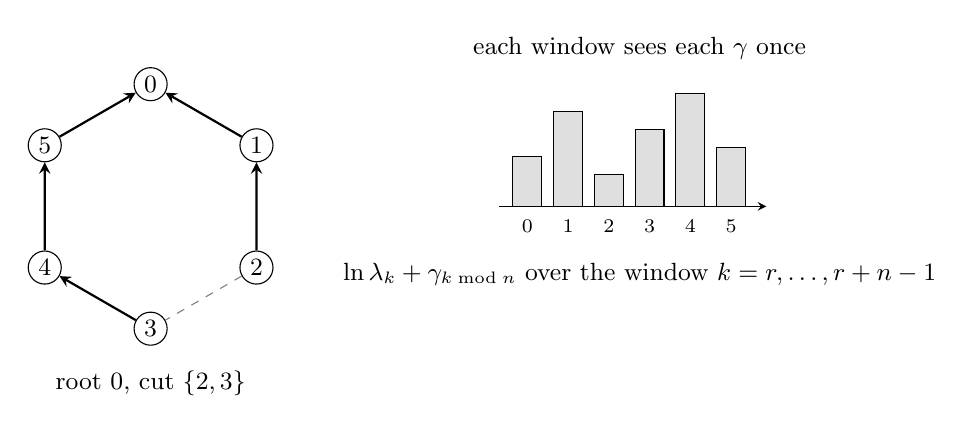
\begin{tikzpicture}[scale=1.15,>=stealth]
\foreach \i in {0,...,5}{\node[circle,draw,inner sep=1.6pt,fill=white] (v\i) at ({90-60*\i}:1.35) {\small\i};}
\draw[->,thick] (v1) -- (v0); \draw[->,thick] (v2) -- (v1);
\draw[->,thick] (v5) -- (v0); \draw[->,thick] (v4) -- (v5);
\draw[dashed,gray] (v2) -- (v3); \draw[->,thick] (v3) -- (v4);
\node at (0,-1.95) {\small root $0$, cut $\{2,3\}$};
\begin{scope}[xshift=5.2cm]
\foreach \k/\h/\lab in {0/0.55/0,1/1.05/1,2/0.35/2,3/0.85/3,4/1.25/4,5/0.65/5}{
  \draw[fill=gray!25] (\k*0.45-1.2,0) rectangle ++(0.32,\h);
  \node at (\k*0.45-1.04,-0.22) {\scriptsize $\lab$};}
\draw[->] (-1.35,0) -- (1.6,0);
\node[align=center] at (0.2,-0.75) {\small $\ln\lambda_k+\gamma_{k\bmod n}$ over the window $k=r,\dots,r+n-1$};
\node[align=center] at (0.2,1.75) {\small each window sees each $\gamma$ once};
\end{scope}
\end{tikzpicture}
\caption{Left: on a cycle, a spanning tree rooted at $r$ deletes one undirected edge and orients the rest towards $r$. Right: its weight is $c_r\lambda_k$ for a sequence $\lambda$ that does not depend on the root (Theorem~\ref{thm:cycle}). Adding one Gumbel variable per edge and taking the maximum over the root's window therefore samples the correct law at every root simultaneously.}
\label{fig:ring}
\end{figure}

\section{Couplings}

\begin{definition}
A \emph{coherent coupling} of rates $W$ is a probability measure $\Theta$ on tree families, supported on UC families, whose $j$-th marginal is $P_j$ for every $j$. A tree family $\sigma$ is \emph{dominant} for rates $\widetilde W$ if, for every $j$, $T_j$ is the unique maximiser of $\widetilde w$ on $\T_j$.
\end{definition}

\begin{lemma}\label{lem:coupling}
If $\Theta$ is a coherent coupling of $W(\lambda)$, then \eqref{eq:six} holds at $\lambda$ with $\theta^\alpha=\Theta(\alpha)$ for every choice of $d$. Moreover $P_j(a\in T)=\sum_\alpha\Theta(\alpha)\,\mathbf 1[a\in T^\alpha_j]$ for all roots $j$ and arcs $a$.
\end{lemma}

\begin{proof}
The weight $w(\sigma)/Z=\prod_kP_k(T_k)$ in \eqref{eq:five} is a product measure with marginals $P_k$. The quantity $G^\sigma_j$ depends on $\sigma$ only through $T_j$, so its average is the same under $\Theta$ and under the product measure. The map $\sigma\mapsto\langle G^\sigma\rangle=\sum_k\pi_kG_k^\sigma$ is a fixed linear combination of these quantities, so its averages also agree. Hence \eqref{eq:five} remains true with $\Theta$ in place of $w(\sigma)/Z$; since $\Theta$ charges only UC families, this is \eqref{eq:six}. The arc statement is the equality of marginals itself: both sides are the probability that the tree at root $j$ contains $a$.
\end{proof}

The arc statement is stronger than \eqref{eq:six}: it places the vector of arc marginals of all roots in the convex hull of the incidence vectors of UC families.

\begin{lemma}[{\cite[Lemma 4]{FH2026}}]\label{lem:dominant}
A tree family that is dominant for some positive rates is UC.
\end{lemma}

\begin{proof}
A family's weight depends only on its multiset. If $\sigma'\neq\sigma$ had $m(\sigma')=m(\sigma)$, then $\widetilde w(\sigma')=\widetilde w(\sigma)$; but $\widetilde w(T'_k)\le\widetilde w(T_k)$ for every $k$ with strict inequality where they differ.
\end{proof}

Consequently, if a random rate vector $\widetilde W$ almost surely has a dominant family whose tree at root $j$ has law $P_j$ for every $j$, the law of that family is a coherent coupling. We call $\widetilde W$ a \emph{perturbation coupling}.

\begin{remark}\label{rem:pifree}
Rescaling all rates leaving a state $v$ by a factor $c$ multiplies $w(T)$ by $c$ for every $T\in\T_j$ with $j\neq v$, and leaves $w(T)$ unchanged for $T\in\T_v$; within each $\T_j$ the factor is common, so it changes $\pi$ but no $P_j$. Fancher and Horowitz used this freedom to hold $\pi$ fixed. Since $\Theta$ depends only on the $P_j$, Theorem~\ref{thm:main} holds for every prescribed $\pi$.
\end{remark}

\section{Cycles}

\begin{theorem}\label{thm:cycle}
Let $G$ be the bidirected cycle on $\Z_n$, $n\ge3$, with $b_v=W(v\to v+1)>0$ and $a_v=W(v\to v-1)>0$. Let $\gamma_0,\dots,\gamma_{n-1}$ be independent standard Gumbel variables, $\gamma_k$ attached to the edge $\{k,k+1\}$, and set $\widetilde W=We^{-\gamma_k}$ on both arcs of $\{k,k+1\}$. Then $\widetilde W$ is a perturbation coupling.
\end{theorem}

\begin{proof}
A tree rooted at $r$ deletes one edge $\{k,k+1\}$ and orients the remaining path towards $r$. Index the deleted edge by the integer $k\in\{r,\dots,r+n-1\}$, reading vertices modulo $n$. The vertices $v=r+1,\dots,k$ then point backwards and $v=k+1,\dots,r+n-1$ point forwards, so
\[
 w_r(k)=\prod_{v=r+1}^{k}a_v\prod_{v=k+1}^{r+n-1}b_v .
\]
Moving the cut from $k-1$ to $k$ changes only vertex $k$, from forwards to backwards, so $w_r(k)/w_r(k-1)=a_k/b_k$ for every root. Define $\lambda_0=1$ and $\lambda_k/\lambda_{k-1}=a_k/b_k$ for all $k\in\Z$, with indices of $a,b$ modulo $n$. Then $w_r(k)=c_r\lambda_k$ with $c_r>0$ independent of $k$. The sequence $\lambda$ is not $n$-periodic: $\lambda_{k+n}/\lambda_k=\prod_v a_v/b_v$, the exponential of minus the cycle affinity, and different roots read different windows of it.

Each tree that deletes $\{k,k+1\}$ uses every other edge exactly once, so $\widetilde w_r(k)=w_r(k)\exp(\gamma_k-\sum_i\gamma_i)$. The heaviest tree at $r$ maximises $\ln\lambda_k+\gamma_{k\bmod n}$ over the window $\{r,\dots,r+n-1\}$. The window contains each residue modulo $n$ exactly once, so these $n$ perturbations are independent standard Gumbel variables. By the Gumbel-max lemma \cite{Yellott1977} the maximiser is almost surely unique and equals $k$ with probability $\lambda_k/\sum_{k'}\lambda_{k'}=P_r(k)$. The same $\gamma$ serve every root.
\end{proof}

The resulting weights are $\theta^\alpha=\Pr(\text{the }\widetilde W\text{-dominant family is }\alpha)$. Sharing the noise between the two arcs of an edge matters. A root's tree uses only one arc of each edge, so independent noise on arcs makes the perturbation of a cut depend on the root; on a five-cycle with random rates its marginals are off by about $0.11$ for the stored seed, with comparable errors for most other random rates.

\section{Cactus networks}

The blocks of a graph are its maximal $2$-connected subgraphs and its bridges. For a block $B$ and a state $j$, let $r_B(j)$ be the vertex of $B$ nearest to $j$; it is $j$ itself when $j\in B$. Let $G[B]$ be the set of arcs lying over edges of $B$.

\begin{lemma}\label{lem:blocks}
Each $G[B]$ is strongly connected. For every $j$, the map $T\mapsto(T\cap G[B])_B$ is a bijection from $\T_j(G)$ onto $\prod_B\T_{r_B(j)}(G[B])$, and $w(T)=\prod_Bw(T\cap G[B])$. Hence $P_j=\bigotimes_BP^B_{r_B(j)}$.
\end{lemma}

\begin{proof}
A directed path between two vertices of $B$ that leaves $B$ must return through the same cut vertex, so the excursion can be removed. For $T\in\T_j(G)$ and $x\in B\setminus\{r_B(j)\}$, the tree path from $x$ to $j$ is a simple path, hence passes through $r_B(j)$ and stays in $B$ until it does. So the arc leaving $x$ lies in $G[B]$ and $T\cap G[B]$ is a spanning arborescence of $B$ rooted at $r_B(j)$. Conversely, take one such arborescence for every block. A vertex $x\neq j$ is the nearest vertex to $j$ in every block containing it except the first block on its path to $j$, so it receives exactly one outgoing arc; the union is a spanning tree glued along the block-cut tree, so it lies in $\T_j(G)$. Distinct blocks have disjoint arc sets.
\end{proof}

\begin{lemma}\label{lem:glue}
If every $G[B]$ has a perturbation coupling, independent perturbations of the blocks form a perturbation coupling of $G$.
\end{lemma}

\begin{proof}
By Lemma~\ref{lem:blocks}, $\widetilde w$ factorises over blocks, so the heaviest tree in $\T_j(G)$ is the union of the heaviest trees in the $\T_{r_B(j)}(G[B])$. Its law is $\bigotimes_BP^B_{r_B(j)}=P_j$.
\end{proof}

\begin{lemma}\label{lem:limits}
(a) Merge each bundle of parallel arcs $u\to v$ into one arc of total rate. If the merged graph has a perturbation coupling, so does $G$. (b) Let $G'$ be a strongly connected spanning subgraph of $G$. If every positive rate vector on $G$ has a coherent coupling, so does every positive rate vector on $G'$.
\end{lemma}

\begin{proof}
(a) For each bundle choose one copy with probability proportional to its rate, independently of everything else; give it the merged perturbed rate and give every other copy half of it. Replacing an unchosen copy by the chosen one strictly increases a tree's weight, so the heaviest tree at each root uses only chosen copies; it is the merged heaviest tree with chosen copies substituted, and it is unique because the merged one is. Under each $P_j$, the copies used by a tree are independent of the merged tree and chosen proportionally to their rates; sharing the choice across roots does not change any single root's law.

(b) Give rate $\varepsilon$ to the arcs of $G$ not in $G'$. As $\varepsilon\to0$ each $P_j$ converges to $P'_j$, because $w(\T_j(G'))>0$. Couplings $\Theta^\varepsilon$ live on the finite set of UC families of $G$; a limit point $\Theta^\ast$ has marginals $P'_j$. These marginals vanish on trees that use a missing arc, so $\Theta^\ast$ charges only families inside $G'$. Such a family that is UC in $G$ is UC in $G'$, because any family with the same multiset also avoids the missing arcs.
\end{proof}

\begin{proof}[Proof of Theorem~\ref{thm:main}]
Let $G^+\supseteq G$ add the missing reverse arc on every edge of the underlying graph; $G^+$ has the same underlying cactus. Merge the parallel arcs of $G^+$ into single arcs. Each block of the merged graph is a bidirected cycle with $n\ge3$, which has a perturbation coupling by Theorem~\ref{thm:cycle}, or a bidirected bridge, whose tree at each root is forced, so the unperturbed rates are a perturbation coupling. Lemma~\ref{lem:glue} gives a perturbation coupling of the merged graph, and Lemma~\ref{lem:limits}(a) lifts it to $G^+$, for every positive rate vector on $G^+$. Lemma~\ref{lem:limits}(b) with $G'=G$ gives a coherent coupling of $G$, and Lemma~\ref{lem:coupling} finishes the proof.
\end{proof}

When every edge carries both arcs and there are no parallel arcs, the coupling is simply the dominant family of $W_a e^{-\gamma_{\bar a}}$ with independent Gumbel variables $\gamma_{\bar a}$ on undirected edges.

\section{What the method cannot do}\label{sec:scope}

\begin{proposition}\label{prop:k4}
For the complete directed graph on four states with the integer rates of Table~\ref{tab:k4}, no coherent coupling exists.
\end{proposition}

\begin{proof}
There are $16$ arborescences per root and $65536$ tree families with $5955$ distinct multisets, of which $346$ occur once. The certificate assigns $y(j,T)\in\{-1,1\}$ to each of the $64$ pairs. Exact rational arithmetic shows $\sum_jy(j,T^\alpha_j)\ge0$ for every UC family $\alpha$, while
\[
 \sum_j\sum_{T\in\T_j}y(j,T)P_j(T)=-\tfrac{74467043099669441}{1314877998480476367}\approx-0.0566.
\]
If a coherent coupling $\Theta$ existed, the second quantity would equal $\sum_\alpha\Theta(\alpha)\sum_jy(j,T^\alpha_j)\ge0$ (weak duality), a contradiction.
\end{proof}

\begin{table}[ht]
\centering\small
\begin{tabular}{cccccccccccc}
\toprule
$0{\to}1$&$0{\to}2$&$0{\to}3$&$1{\to}0$&$1{\to}2$&$1{\to}3$&$2{\to}0$&$2{\to}1$&$2{\to}3$&$3{\to}0$&$3{\to}1$&$3{\to}2$\\
\midrule
2&50&100&10&20&1&100&2&5&2&100&100\\
\bottomrule
\end{tabular}
\caption{Rates of the four-state obstruction.}
\label{tab:k4}
\end{table}

The obstruction propagates to every network that contains $K_4$ as a minor. For a connected simple graph $\Gamma$ let $\vec\Gamma$ be the network with both arcs on every edge, and say that a network has property $\mathsf{C}$ if every positive rate vector on it has a coherent coupling.

\begin{lemma}\label{lem:minor}
Property $\mathsf{C}$ passes from a network $G$ to each of the following.
(a) A strongly connected spanning subgraph $G'$ of $G$.
(b) $G-x$, where $x$ is a state joined only to one state $u$, by the two arcs $x\to u$ and $u\to x$.
(c) The network $G_x$ obtained by suppressing a state $x$ whose only arcs are $x\rightleftarrows u$ and $x\rightleftarrows v$, where $u\neq v$ are not adjacent: delete $x$ and add the arcs $u\to v$ and $v\to u$.
\end{lemma}

\begin{proof}
(a) is Lemma~\ref{lem:limits}(b). In (b) and (c) we take target rates on the smaller network, choose rates on $G$, take a coherent coupling $\Theta$ of $G$, and push it forward along a map $\kappa$ from arborescences of $G$ rooted at $j\neq x$ to arborescences of the smaller network rooted at $j$; the tree at root $x$ is discarded.

(b) Every arborescence rooted at $j\neq x$ contains $x\to u$ and not $u\to x$; deleting $x\to u$ is a bijection onto $\T_j(G-x)$ that divides every weight by $W(x\to u)$, so $\kappa$ pushes $P_j$ to $P^{G-x}_j$.

(c) Given rates $c_{uv},c_{vu}$ on the new arcs, put $W(x\to u)=W(x\to v)=1$, $W(u\to x)=2c_{uv}$ and $W(v\to x)=2c_{vu}$. In an arborescence rooted at $j\neq x$, the state $x$ is either a leaf, attached by $x\to u$ or $x\to v$, or lies on a path $u\to x\to v$ or $v\to x\to u$ (it cannot receive arcs from both neighbours, since its out-arc and the reverse arc would form a $2$-cycle); let $\kappa$ delete the arc out of a leaf $x$ and replace $u\to x\to v$ by $u\to v$ and $v\to x\to u$ by $v\to u$. A tree of $G_x$ of weight $w$ that uses neither new arc has two preimages, each of weight $w$; one that uses $u\to v$ has the single preimage of weight $W(u\to x)W(x\to v)\,w/c_{uv}=2w$, and similarly for $v\to u$. Every tree of $G_x$ therefore receives total weight $2w$, and $\kappa$ pushes $P_j$ to $P^{G_x}_j$.

In both cases the push-forward $\kappa_\ast\Theta$, applied root by root to the roots $j\neq x$, has the right marginals, and it remains to show that $\kappa$ maps UC families to UC families. Let $\sigma$ be a family of $G$ and suppose a family $\tau\neq\kappa(\sigma)$ of the smaller network has the same multiset as $\kappa(\sigma)$. Lift $\tau$ to a family $\tau'$ of $G$: keep $\sigma_x$ at the root $x$; in (b) add $x\to u$ to every tree; in (c) replace $u\to v$ by $u\to x\to v$ and $v\to u$ by $v\to x\to u$, and attach $x$ as a leaf in the remaining trees, using $x\to u$ in exactly as many of them as $\sigma$ does. Since $\tau$ and $\kappa(\sigma)$ use $u\to v$ and $v\to u$ equally often, they have equally many trees in which $x$ is a leaf, so this is possible, and then $\tau'$ and $\sigma$ use every arc of $G$ equally often: arcs away from $x$ because $\tau$ and $\kappa(\sigma)$ have the same multiset, $u\to x$ and $v\to x$ because they occur exactly on the paths replacing $u\to v$ and $v\to u$, and $x\to u$, $x\to v$ by the choice of leaves. Each lifted tree is an arborescence, and $\kappa$ undoes the lift, so $\tau'_j=\sigma_j$ for all $j\neq x$ would give $\tau=\kappa(\sigma)$. Hence $\tau'\neq\sigma$ and $\sigma$ is not UC.
\end{proof}

\begin{theorem}\label{thm:minor}
If a connected graph $\Gamma$ has a $K_4$ minor, some positive rates on $\vec\Gamma$ admit no coherent coupling.
\end{theorem}

\begin{proof}
Since $K_4$ has maximum degree $3$, a graph with a $K_4$ minor contains a subdivision $H$ of $K_4$ as a subgraph; this is the standard fact that a minor of maximum degree at most $3$ is a topological minor \cite[Section~1.7]{Diestel2017}. Add to $H$ a spanning forest joining the other vertices of $\Gamma$ to $H$; the result $\Gamma'$ is a connected spanning subgraph of $\Gamma$ consisting of $H$ with trees attached. If $\vec\Gamma$ had property $\mathsf C$, then so would $\vec\Gamma'$ by Lemma~\ref{lem:minor}(a), and so would $\vec H$ after removing, one at a time, a vertex outside $H$ at maximal distance from $H$, which is a leaf, by Lemma~\ref{lem:minor}(b). The neighbours of a subdividing vertex of $H$ are never adjacent, since every cycle of a subdivision of $K_4$ through a subdividing vertex has length at least $4$, being a subdivided cycle of $K_4$ with at least one extra vertex; each suppression yields a subdivision of $K_4$ with one fewer subdividing vertex. Suppressing subdividing vertices one at a time by Lemma~\ref{lem:minor}(c) gives property $\mathsf C$ for $\vec K_4$, contradicting Proposition~\ref{prop:k4}.
\end{proof}

For $K_4$ with one edge subdivided we also replayed the construction of Lemma~\ref{lem:minor}(c) exactly: contraction maps each of the $984$ UC families to a UC family of $K_4$, and the lifted certificate is nonnegative on all $984$ UC families among the $24^5$ tree families and has the same negative expectation.

Proposition~\ref{prop:k4} says that Lemma~\ref{lem:coupling} cannot prove the conjecture for $K_4$. It does not refute the conjecture. There is a chain of requirements on a measure $\Theta$ on UC families, each implying the next: (i) root marginals $P_j$ for every $j$ (a coherent coupling); (ii) arc marginals $P_j(a\in T)$ for every $j$ and $a$, as in Lemma~\ref{lem:coupling}; (iii) one $\Theta$ satisfying \eqref{eq:six} for all $d$ at once, which only asks for the centred arc marginals $P_j(a\in T)-\sum_k\pi_kP_k(a\in T)$; (iv) for each $d$ separately, some $\Theta$ satisfying \eqref{eq:six}, which is the conjecture. Proposition~\ref{prop:k4} rules out (i) only; we have not proved that any of the later implications is strict. In our searches the conjecture survives. Gradient ascent of random linear functionals of the response, with unbounded log-rates, never exceeded the UC bound on $K_4$ (150 runs) or, for pairs of roots, on $K_5$ (150 runs); exploratory runs on several other five-state graphs agreed. In exploratory computations that are not part of the verification scripts, critical points constructed directly on $K_4$ were all saddles, and the vector of arc marginals stayed inside the convex hull of UC incidence vectors, so (ii) held at the sampled rates; on $K_4$ it touches the boundary at reversible rates, where all roots share one undirected spanning-tree law.

Theorem~\ref{thm:minor} shows that the coupling method can at most reach graphs without a $K_4$ minor, whose blocks are series-parallel, and Theorem~\ref{thm:main} reaches the cacti among them. We conjecture that it reaches all of them: linear programs found coherent couplings for every sampled rate vector on the four-state diamond (two triangles sharing an edge), on $K_{2,3}$ and on a five-cycle with a chord, and failed for some sampled rates on $K_4$ and on $K_4$ with one edge subdivided, consistent with Theorem~\ref{thm:minor}. The edge-Gumbel perturbation is exact on cacti, but its error is about $0.06$ on the diamond, so series-parallel networks would need a different construction.

\textbf{Priority.} We searched arXiv to October 2026, including later versions of \cite{FH2026}, Zenodo, GitHub problem trackers and the authors' pages, and found no proof, partial proof or counterexample. The Gumbel-max lemma \cite{Yellott1977} and perturb-and-MAP sampling \cite{PapandreouYuille2011,Maddison2014} are classical. Gumbel perturbations of spanning trees and arborescences are used in machine learning as relaxations and approximate samplers \cite{Paulus2020,Struminsky2021}, without exactness or coupling across roots. Exactness of perturb-and-MAP for full-order perturbations is classical \cite{HazanJaakkola2012}; our perturbation has only one variable per edge, and exactness comes from the window structure of cycles. Couplings of the root laws by themselves are easy, for instance by running the cycle-popping algorithm of Propp and Wilson \cite{ProppWilson1998} for every root on common stacks, but in our experiments such couplings charge non-UC families. We know of no earlier coupling of all rooted laws supported on UC families.

\section{Verification}

The theorem rests on the written proofs. Standard-library scripts check the cycle identity $w_r(k)/w_r(k-1)=a_k/b_k$ exactly for $n\le8$. They also check block factorisation exactly on five cacti and, for sampled rates, that dominant families are UC. A separate script enumerates all $K_4$ tree families from scratch and replays the Farkas certificate in rational arithmetic, and a third replays the suppression step of Lemma~\ref{lem:minor}(c) on $K_4$ with one edge subdivided. A floating-point script reproduces the Monte Carlo, linear-programming and search evidence of Section~\ref{sec:scope}. None of this is formalised in Lean.

\bibliographystyle{amsplain}
\bibliography{references}
\end{document}
